% diagram-final-muse.tex -- consensus figure for Section 3 (Hybrid level step).
% Standalone: compile with  pdflatex diagram-final-muse.tex
% to produce the PDF included as figs/approach-hybrid.pdf.
%
% Consensus design (Round 4): two swim lanes (GPU top, host/CPU bottom),
% time left-to-right, one staged copy path between them, a dashed
% "concurrent" link between the next GPU level and the CPU subtree
% tasks, and a single full-width shared-store bar at the bottom.
% Deliberately omitted: kernel names, tile size, buffer capacities,
% timings, a socket/NUMA diagram (only a one-line label on the pinned
% buffers), pruning, and any second panel for GPU-Based (caption: m=1).
\documentclass[tikz,border=4pt]{standalone}
\usepackage{tikz}
\usetikzlibrary{arrows.meta,positioning,fit,backgrounds,shapes.geometric}

\begin{document}
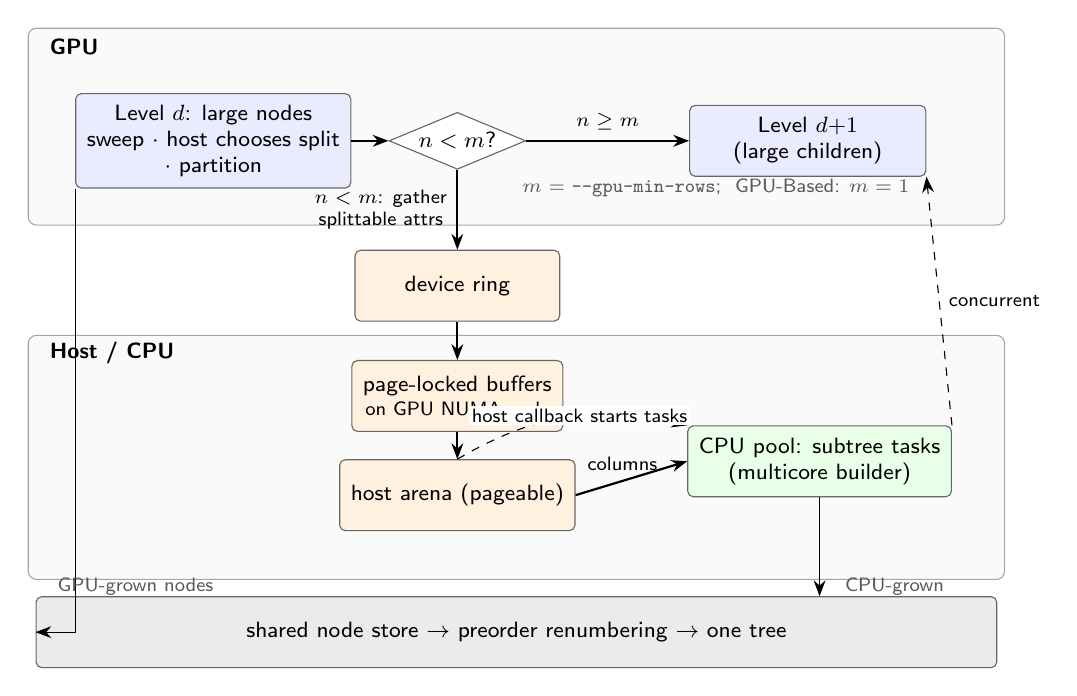
\begin{tikzpicture}[
  font=\sffamily\footnotesize,
  >={Stealth[length=2mm]},
  lane/.style={draw=black!35, fill=black!2, rounded corners=3pt},
  box/.style={draw=black!60, rounded corners=2pt, align=center,
              inner sep=4pt, minimum height=9mm},
  gpu/.style={box, fill=blue!8},
  buf/.style={box, fill=orange!12},
  cpu/.style={box, fill=green!9},
  solid/.style={->, thick},
  ctrl/.style={->, dashed},
  lbl/.style={font=\sffamily\scriptsize, align=center},
  tiny/.style={font=\sffamily\scriptsize, text=black!65},
]

% ---------- lanes ----------
\draw[lane] (0,3.55) rectangle (12.4,6.05);
\node[anchor=west, font=\sffamily\footnotesize\bfseries] at (0.15,5.82)
  {GPU};
\draw[lane] (0,-0.95) rectangle (12.4,2.15);
\node[anchor=west, font=\sffamily\footnotesize\bfseries] at (0.15,1.92)
  {Host / CPU};

% ---------- GPU lane ----------
\node[gpu, minimum width=30mm] (level) at (2.35,4.62)
  {Level $d$: large nodes\\ sweep $\cdot$ host chooses split\\ $\cdot$ partition};
\node[draw=black!60, diamond, aspect=2.4, inner sep=1pt, fill=white]
  (fork) at (5.45,4.62) {$n<m$?};
\node[gpu, minimum width=30mm] (next) at (9.9,4.62)
  {Level $d{+}1$\\ (large children)};

\draw[solid] (level) -- (fork);
\draw[solid] (fork) -- node[lbl, above] {$n \ge m$} (next);

% ---------- copy path ----------
\node[buf, minimum width=26mm] (ring) at (5.45,2.78)
  {device ring};
\node[buf, minimum width=26mm] (pin) at (5.45,1.38)
  {page-locked buffers\\[-1pt] {\scriptsize on GPU NUMA node}};
\node[buf, minimum width=26mm] (arena) at (5.45,0.12)
  {host arena (pageable)};

\draw[solid] (fork.south) -- node[lbl, left] {$n<m$: gather\\ splittable attrs} (ring);
\draw[solid] (ring) -- (pin);
\draw[solid] (pin) -- (arena);

% ---------- CPU lane ----------
\node[cpu, minimum width=30mm] (tasks) at (10.05,0.55)
  {CPU pool: subtree tasks\\ (multicore builder)};

\draw[solid] (arena.east) -- node[lbl, above, pos=0.42] {columns} (tasks.west);
\draw[ctrl] (arena.north) to[bend left=22]
  node[lbl, fill=white, inner sep=1pt, pos=0.55] {host callback starts tasks}
  (tasks.north west);

% overlap: next GPU level runs while CPU tasks grow handed-off subtrees
\draw[ctrl] (tasks.north east) -- (next.south east)
  node[lbl, right, pos=0.5] {concurrent};

% ---------- shared store ----------
\node[box, fill=black!8, minimum width=122mm] (store) at (6.2,-1.62)
  {shared node store $\rightarrow$ preorder renumbering $\rightarrow$ one tree};

\draw[->] (level.south west) |- (store.west);
\node[tiny, anchor=south west] at (0.25,-1.28) {GPU-grown nodes};
\draw[->] (tasks.south) -- (store.north -| tasks.south);
\node[tiny, anchor=south west] at (10.25,-1.28) {CPU-grown};

% threshold / GPU-only note
\node[tiny, align=left, anchor=west] at (6.15,4.02)
  {$m$ = \texttt{--gpu-min-rows};\ \ GPU-Based: $m=1$};

\end{tikzpicture}
\end{document}
